\documentclass[12pt, letterpaper]{article}

\usepackage[utf8]{inputenc}
\usepackage{float}
\usepackage{systeme}
\usepackage{amsmath}
\usepackage{amssymb}
\usepackage{enumitem}
\usepackage{amsfonts}
\usepackage{amsthm}
\usepackage{graphicx}
\usepackage[colorinlistoftodos]{todonotes}
\usepackage{pifont}
\usepackage{mdframed,color}
\usepackage[letterpaper, left=3cm, right=3cm, top=3cm, bottom=3cm]{geometry}
\newcommand{\Z}{\mathbb{Z}}
\newcommand{\N}{\mathbb{N}}
\newcommand{\C}{\mathbb{C}}
\newcommand{\Q}{\mathbb{Q}}
\newcommand{\R}{\mathbb{R}}
\newcommand{\F}{\mathbb{F}}
\newtheoremstyle{statement}{3pt}{3pt}{}{}{\bfseries}{:}{.5em}{}

\theoremstyle{statement}
\newtheorem*{atmProp}{Proposition}

\theoremstyle{statement}
\newtheorem*{atmStat}{Statement}

\newenvironment{atmProof}{\noindent\ignorespaces\paragraph{Proof:}}{\hfill \ding{122}\par\noindent}

\newenvironment{Solution}{\noindent\ignorespaces\paragraph{Solution:}}{\hfill \ding{122}\par\noindent}

\newcount\arrowcount
\newcommand\arrows[1]{
        \global\arrowcount#1
        \ifnum\arrowcount>0
                \begin{matrix}
                \expandafter\nextarrow
        \fi
}

\newcommand\nextarrow[1]{
        \global\advance\arrowcount-1
        \ifx\relax#1\relax\else \xrightarrow{#1}\fi
        \ifnum\arrowcount=0
                \end{matrix}
        \else
                \\
                \expandafter\nextarrow
        \fi
}

\newcommand{\func}[2]{\operatorname{#1}(#2)}
\newcommand{\trans}[2]{\func{#1}{\Vec{#2}}}

\title{Mastery Homework 5}
\author{Rafael Laya}
\date{Fall 2018}

\begin{document}
    \maketitle
    
    \section*{Section 2.3}
    \subsection*{Problem 20}
    \begin{atmStat}
    If nxn matrices $E$ and $F$ have the property that $EF=I$, then $E$ and $F$ commute. Explain why.
    \end{atmStat}
    \begin{Solution}
    Because if $EF=I$ then we know by the Invertible Matrix Theorem and by the result or problem 27 solved in fundamental homework that they are inverses of each other and therefore $E$ and $F$ multiply and result on the identity whether it is $EF$ or $FE$. Let's show this: \\
    
    Let $E$ and $F$ be two matrices of order nxn. Suppose that $EF=I$ where $I$ is the identity matrix of order nxn. Applying the Invertible Matrix Theorem we know that $F$ is invertible. Consider: 
    $$EF=I$$
    Multiply both sides of the equality above by $F^{-1}$ on the right:
    \begin{align*}
        (EF)F^{-1} &= IF^{-1} \\
        E(FF^{-1}) &= F^{-1} \\ 
        E(I) &= F^{-1} \\ 
        E &= F^{-1} \\
    \end{align*}
    Multiply both sides of the equality above by $F$ on the left:
    \begin{align*}
        E &= F^{-1} \\
        FE &= FF^{-1} \\
        FE &= I
    \end{align*}
    Therefore, 
    $$EF=I=FE$$
    Which shows that $E$ and $F$ commute.
    \end{Solution}
    
    \subsection*{Problem 32}
    \begin{atmStat}
    Suppose $A$ is a nxn matrix with the property that the equation $A\Vec{x}=\Vec{0}$ has only trivial solution. Without using the Invertible Matrix Theorem, explain directly why the equation $A\Vec{x}=\Vec{b}$ must have a solution for each $\Vec{b}$ in $\R^n.$
    \end{atmStat}
    \begin{Solution}
    Simply because if $A\Vec{x}=\Vec{0}$ has only trivial solution we know that the row reduced echelon form of $A$ must not have a row of zero-es and therefore the system will be consistent for any vector $\Vec{b}$ that we use in the augmented column of $\begin{bmatrix} A && \Vec{b}\end{bmatrix}$ with this argument in mind:\\
    
    Let $A$ be a nxn matrix with the property that $A\Vec{x}=\Vec{0}$ has only trivial solution. Then, due to theorem 2 in chapter 1 we know that the matrix $A$ must not have any free variables since the system is consistent and it has unique solution. Because $A$ has $n$ columns it must have $n$ pivot positions that correspond to $n$ basic variables. $A$ must also have a pivot in every row since it has $n$ pivots and $n$ rows, using theorem 4 from chapter 1 we know that there is a solution for each $\Vec{b}\in\R^n$.
    \end{Solution}
    
    \subsection*{Problem 38}
    \begin{atmStat}
    Suppose a linear transformation $\operatorname{T}:\R^n\longrightarrow\R^n$ has the property that $\trans{T}{u}=\func{T}{\Vec{v}}$ for some pair of distinct vectors $\Vec{u}$ and $\Vec{v}$ in $\R^n$. Can $\operatorname{T}$ map $\R^n$ onto $\R^n$? Why or Why not?
    \end{atmStat}
    \begin{Solution}
    Let $\operatorname{T}:\R^n\longrightarrow\R^n$ be a linear transformation. Assume $\trans{T}{u}=\trans{T}{v}$ for some $\Vec{u},\Vec{v}\in\R^n$ with $\Vec{u}\neq\Vec{v}$. By theorem 10 in chapter 1 we know that there exists a matrix $A$ such that: 
    
    $$\trans{T}{x}=A\Vec{x}$$
    For all $\Vec{x}\in\R^n$. By assumption the transformation $\operatorname{T}$ is not one-to-one, since $\trans{T}{u}=\trans{T}{v}$ with $\Vec{u}\neq\Vec{v}$. Using the Invertible Matrix Theorem, since $\operatorname{T}$ is not one-to-one the linear transformation $\operatorname{T}$ does not map $\R^n$ onto $\R^n$.
    \end{Solution}
    
    \section*{Section 3.1}
    \subsection*{Problem 41}
    \begin{atmStat}
    Let $\Vec{u}=\begin{bmatrix} 3 \\0 \end{bmatrix}$ and $\Vec{v}= \begin{bmatrix} 1 \\ 2 \end{bmatrix}$. Compute the area of the parallelogram determined by $\Vec{u}, \Vec{v}, \Vec{u}+\Vec{v}$, and $\Vec{0}$, and compute the determinant of $\begin{bmatrix} \Vec{u} && \Vec{v}\end{bmatrix}$. How do they compare? Replace the first entry of $\Vec{v}$ by an arbitrary number $x$, and repeat the problem. Draw a picture and explain what you find.
    \end{atmStat}
    \begin{Solution}
    First draw a picture of the parallelogram determined by $\Vec{u}, \Vec{v}, \Vec{u}+\Vec{v}, \Vec{0}$
    
    \begin{figure}[H]
        \centering
        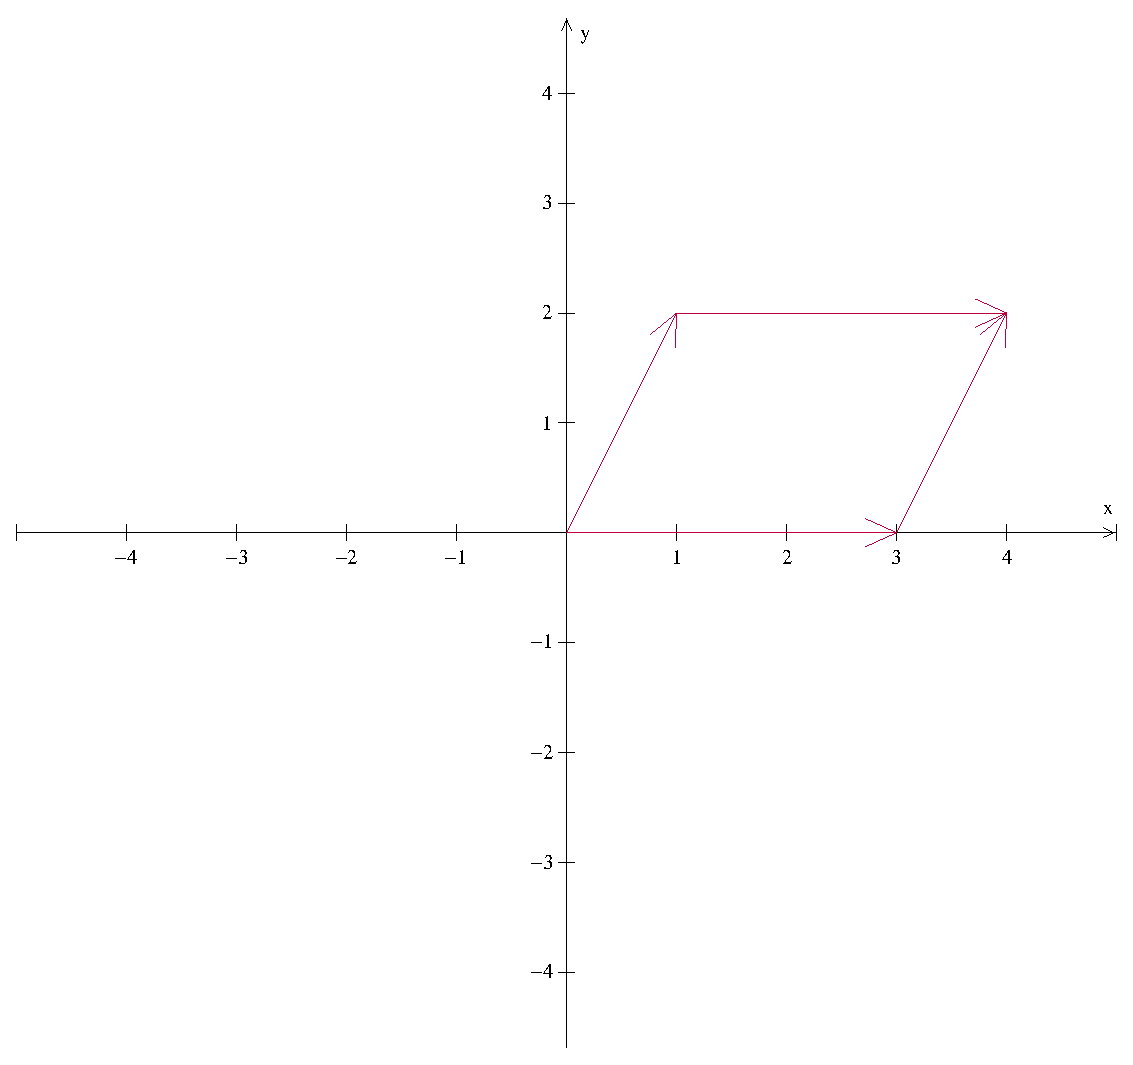
\includegraphics[scale=0.5]{vectors}
        \caption{Parallelogram determined by $\Vec{u}, \Vec{v}, \Vec{u}+\Vec{v}, \Vec{0}$}
        \label{vectors1}
    \end{figure}
    Since the base of the parallelogram is $3$ and height $2$ its area is $3\cdot2=6$. Let's calculate the determinant of $\begin{bmatrix} \Vec{u} && \Vec{v}\end{bmatrix}$
    
    $$
    \begin{vmatrix}
    3 & 1 \\
    0 & 2 \\
    \end{vmatrix}
    = 3(2) - 1(0) = 6
    $$
    They compare by being exactly the same. That is, in this case: $\begin{vmatrix} \Vec{u} & \Vec{v} \end{vmatrix}=6=$ Area of the parallelogram spanned by $\Vec{v}, \Vec{u}, \Vec{v}+\Vec{u}, \Vec{0}$
    
    Replacing the first entry of $\Vec{v}$ by a number $x$ we have: 
    
    \begin{figure}[H]
        \centering
        \includegraphics[scale=0.5]{Untitled}
        \caption{The parallelogram with a few different values of $x$}
        \label{vectors2}
    \end{figure}
    
    Notice that no matter the value of $x$, the parallelogram is always of base three and height two, therefore its area is always $6$. Also: 

    $$
    \begin{vmatrix}
    3 & x \\
    0 & 2 \\
    \end{vmatrix}
    = 3(2) - x(0) = 6
    $$
    \end{Solution}
    
    This gives us a hint that the determinant $\begin{vmatrix} \Vec{u} & \Vec{v}\end{vmatrix} $ is closely related to the area of the paralleogram spanned by the vectors $\Vec{u}, \Vec{v}$. Namely, $\begin{vmatrix} \Vec{u} && \Vec{v}\end{vmatrix}$ is exactly the area of the parallelogram spanned by $\Vec{u}, \Vec{v}$ (In reality we have to add absolute value to the determinant because it might turn out negative, using knowledge from Calculus 3).
    
    \section*{Section 3.2}
    \subsection*{Problem 34}
    \begin{atmStat}
    Let $A$ and $P$ be square matrices, with $P$ invertible. Show that $\det(PAP^{-1})=\det(A)$.
    \end{atmStat}
    \begin{Solution}
    Suppose $A$ and $P$ are matrices of nxn with $P$ invertible. That is, there exists $P^{-1}$ such that:
    
    $$
    PP^{-1} = I
    $$
    Where $I$ is the identity matrix of order nxn. We also know that: 
    $$
    \det(PP^{-1}) = \frac{1}{\det(P)}
    $$
    Now, using the multiplicative property of determinants:
    
    \begin{align*}
        \det(PAP^{-1}) &= det(PA)\dot\det(P^{-1}) \\
        &= \det(P)\det(A)\frac{1}{\det(P^{-1})} \\
        &= \det(A)\left( \det(P) \frac{1}{\det(P^{-1})}\right) \\
        &= \det(A)(1) \\
        &= \det(A)
    \end{align*}
    Which is precisely what we wanted to show.
    \end{Solution}
    
    \subsection*{Problem 36}
    \begin{atmStat}
    Find a formula for $\det(rA)$ when $A$ is a nxn matrix.
    \end{atmStat}
    \begin{Solution}
    Let $r\in\R$ and $A$ be a matrix of nxn. Then, define $R$ as the diagonal matrix of nxn where the entries in the diagonal are $r$. Because $R$ is diagonal matrix, by theorem its determinant is the product along the diagonal (a diagonal matrix is also triangular matrix). Because $R$ is of nxn, it has $n$ entries on its diagonal. Therefore $\det(R)=r^n$. Let's denote $a_{ij}$ as the entry in $A$ at row $i$, column $j$. Notice, however that $rA=RA$, 
    $$
    \begin{bmatrix}
    r & 0 & \dots & 0 \\
    0 & r & \dots & 0 \\
    \vdots & \vdots & \ddots & \vdots \\
    0 & 0 & \dots & r
    \end{bmatrix}
    \begin{bmatrix}
    a_{11} & \dots & a_{1n} \\
    \vdots & & \vdots \\
    a_{n1} & \dots & a_{nn}
    \end{bmatrix}
    =
    \begin{bmatrix}
    ra_{11} & \dots & ra_{1n} \\
    \vdots & & \vdots \\
    ra_{n1} & \dots & ra_{nn}
    \end{bmatrix}
    =
    r
    \begin{bmatrix}
    a_{11} & \dots & a_{1n} \\
    \vdots & & \vdots \\
    a_{n1} & \dots & a_{nn}
    \end{bmatrix}
    $$
    
    Because $R$ is the result of multiplying every row of the identity matrix of order nxn by $r$. Now, using the multiplicative propery of determinants:
    
    \begin{align*}
       \det(rA) &= \det(RA) \\
       &= \det(R)\det(A) \\
       &= r^n\det(A)
    \end{align*}
    
    Which is the formula we wanted.
    \end{Solution}
    
\end{document}
